%______________________________________________________________________________________________________________________
% @brief    LaTeX2e Resume for Kamil K Wojcicki
\documentclass[margin,line]{resume}
\usepackage[latin1]{inputenc}
\usepackage{graphics}
\usepackage{amsmath,amssymb}
\usepackage{gensymb}
\usepackage{amsthm}
\usepackage{wrapfig,lipsum,booktabs}
\usepackage{caption}
\usepackage{subcaption}
\usepackage{tabulary}
\usepackage{epigraph}
\usepackage{mwe}
\usepackage[autostyle]{csquotes} 
\usepackage{lipsum,lmodern}
\usepackage[skins]{tcolorbox}
\usepackage{pgf,tikz}
\usetikzlibrary{arrows,shapes,backgrounds,fit}
\usetikzlibrary{arrows,automata}

\usepackage{fancyvrb}
\usepackage{listings}
\usepackage{color}
\usepackage{eurosym}
%______________________________________________________________________________________________________________________
\begin{document}
\name{\Large Simon Holmbacka. PhD -- Resume\flushright{19 June 2018}}
\begin{resume}
\begin{picture}(320,0)
\put(320,-160){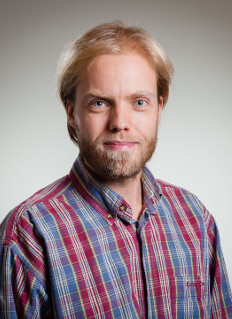
\includegraphics[scale=0.5]{simon.jpg}}
\end{picture}
    %__________________________________________________________________________________________________________________
    % Contact Information
    \section{\mysidestyle Contact\\Information}

%     Embedded Systems Laboratory                         	     \vspace{0mm}\\\vspace{0mm}%
%     Faculty of Science and Engineering                           \vspace{0mm}\\\vspace{0mm}%
%     \AA{}bo Akademi University, Finland			       		\vspace{0mm}\\\vspace{-4.5mm}%
    
\small{
    Haagantie 62			\vspace{0mm}\\\vspace{0mm}%
    20380 Turku, Finland		\vspace{0mm}\\\vspace{0mm}%
    Tel: +358 50 5310467		\vspace{0mm}\\\vspace{0mm}%
    Email: sholmbac@abo.fi		\vspace{0mm}\\\vspace{0mm}%
    Gender: male			\vspace{0mm}\\\vspace{0mm}%
    Time of birth: 24.01.1986		\vspace{0mm}\\\vspace{0mm}%
    Place of birth: Jakobstad, Finland	\vspace{0mm}\\\vspace{0mm}%
    Nationality: Finnish		\vspace{0mm}\\\vspace{-4.5mm}%
    }
\vspace{1.5cm}
\section{\mysidestyle Position}
    \textbf{AI Researcher}	\hfill \textbf{May 2017 -- }\vspace{0mm}\\\vspace{0mm}%
    Elisa Oyj.\\
    Task: \textit{Mobile network optimization using deep learning}\\  
    \textbf{Senior Researcher}	\hfill \textbf{June 2017 -- }\vspace{0mm}\\\vspace{0mm}%
    University of Turku\\
    Task: \textit{MooC developer for online education}\\  
\vspace{-0.5cm}
    
\section{\mysidestyle Education}

    \textbf{\AA{}bo Akademi University}, Finland \vspace{2mm}\\\vspace{1mm}%
    \textsl{Doctor of Technology in Computer Engineering (26 Jan. 2016, Turku, Finland)} \hfill \textbf{ 2011 -- 2015}\vspace{-3mm}\\\vspace{-1mm}%
    \begin{list2}
        \item Faculty: Science and Engineering
	\item Major: Embedded Computer Systems
	\item Minor: Software Engineering
	\item Minor: University Pedagogics
	\item Thesis: \textit{Energy-Aware Software for Many-Core Systems} \textbf{Grade:} Honorary Grade
	\item Reference: Prof. Johan Lilius \textit{johan.lilius@abo.fi}
    \end{list2}\vspace{-1.5mm}
    \textsl{Master of Science in Computer Engineering (31 Mar. 2011, Turku, Finland)} \hfill \textbf{ 2009 -- 2011}\vspace{-3mm}\\\vspace{-1mm}%
    \begin{list2}
        \item Institution: Information Technologies
	\item Major: Embedded Computer Systems
	\item Minor: Control Engineering
	\item Minor: Software Engineering
	\item Thesis: \textit{Task Migration in Virtualized Multi-Core Real-Time Systems} \textbf{Grade:} 5/5
    \end{list2}\vspace{-1.5mm}
    \textsl{Bachelor of Science in Computer Engineering (6 Oct. 2009, Turku, Finland)} \hfill \textbf{ 2006 -- 2009}\vspace{-3mm}\\\vspace{-1mm}%
    \begin{list2}
        \item Institution: Information Technologies
	\item Major: Embedded Computer Systems
	\item Minor: Software Engineering
    \end{list2}\vspace{-1.5mm}

% \section{\mysidestyle Research\\Interests}
% Energy-Aware Software, Power Management, Parallel Programming, Many-Core Systems, Control Theory    
%    
%     
\section{\mysidestyle About me}
I come from the small city of Jakobstad in the mid west of Finland from which I moved to Turku to study computer engineering in 2006.
I completed my Master's degree in 5 years (2006 -- 2011) and my PhD in 4 years (2011 -- 2015) from \AA{}bo Akademi University in Turku, Finland.

\hspace{-2.0cm} \textit{Technical}\\
I have worked extensively in the areas of embedded systems, runtime systems, power management and many-core platforms, which includes foremost low level system programming (usually in C), and lately I have been using Python more.
Furthermore I have experience in other object oriented programming languages, mostly C++ and Java, and I have of course stumbled upon some Java script, xml and assembly programming.
I have worked with system modeling, mathematical optimization and control theory including NLP optimization, digital filtering, plane fitting methods, control theory and its underlying mathematics. 
This means that I have very good knowledge of Matlab, its toolboxes and system simulation in Simulink.
On the hardware side, I have excellent knowledge of ARM and Intel platforms in particular, and system/kernel programming using Linux. 
I have been hacking with the Linux kernel since I was 16 years old and know this world in and out.
On further lower level I have worked with real-time operating systems like FreeRTOS during my PhD and I have also build many hobby projects from scratch using micro controllers such as an audio synthesizer complete with a midi interface and USB driver running on an 8-bit AVR.
I am currently working with big data deep learning using Tensorflow/Keras and R, and optimization of deep learning models in Opentuner.
\clearpage

\hspace{-2.0cm} \textit{Project Work}\\
In the 4 years of making my PhD I have published over 15 international peer reviewed scientific articles, one of which I received the best paper award for in 2014. 
I worked in the European FP-7 project RECOMP from 2011 -- 2014 and in the national Tekes project ParallaX from 2014 -- 2016, in which I worked together with universities and
international IT companies like Wittenstein ltd., UK and Seven Solutions, Spain on programming and integration tasks.
I am a very good team worker, which has shown in co-operations with 7 different universities in 4 countries during this time for my thesis, and outside of my thesis I have published work together with 12 different institutions and co-authored work together with over 30 people.
I have visited more than 30 countries in my thesis work, and I find it very easy to join a team and start working on new projects with new people. 

\hspace{-2.0cm} \textit{Languages}
\quad \qquad 
\includegraphics[scale=0.1]{flags.png}
\vspace{-0.5cm}
\begin{itemize}
 \item Swedish: Mother tongue 
 \item Finnish: Conversational
 \item English: Fluent
 \item German: Conversational
\end{itemize}
\hspace{-2.0cm} \textit{Pedagogics}\\
Education wise, I have been lecturing university courses in English since 2013 and completed university pedagogics as a minor subject.
I created two online education MooCs on coursera.org from scratch in the EIT Digital project in 2015 -- 2018, which are now freely available on Coursera and has thousands active students.\\ 

\hspace{-2.0cm} \textit{About Simon}\\
I would describe myself as a person who takes the initiative, gets things started and gets things done. 
I have a very good working discipline with regard to time and responsibility, and \textit{I always do the work today instead of leaving it until tomorrow}! 
I always start a task well on time, and I keep the promised timelines whether it is a question of delivering C code, an article, a presentation, course material or a PhD thesis.\\ 
My hobbies are traveling, gardening, skiing, hiking, driving, workout, watching airplanes and Trump-Russia investigation.


\section{\mysidestyle Teaching\\Experience}
  \textbf{Course administrator}: EIT Digital Online Coursera\\ \textit{Embedded Hardware and Operating Systems} \hfill \textbf{2018}\\
  \color{blue}https://www.coursera.org/learn/embedded-operating-system/\color{black}\\
  \textbf{Course creator}: EIT Digital Online Coursera\\ \textit{Autonomous Runway Detection for IoT} \hfill \textbf{2017}\\
  \color{blue}https://www.coursera.org/learn/embedded-systems-larger/\color{black}\\
  \textbf{Course creator and lecturer}: EIT Digital Online Coursera\\ \textit{Development of Real-Time Systems} \hfill \textbf{2016}\\
  \color{blue}https://www.coursera.org/learn/real-time-systems/\color{black}\\\\
  \textbf{Course lecturer}: Real-Time Systems \AA{}bo Akademi University \hfill \textbf{2012 -- 2017}\\
  \textbf{Advisor and examiner for thesis work}: \AA{}bo Akademi University \hfill \textbf{2012 -- 2016}\\
  \textbf{Pr\"{u}fer f\"{u}r Abschlussarbeiten}: FernUniversit\"{a}t in Hagen \hfill \textbf{2015 -- 2016}\\
  \textbf{Course assistant}: Multimedia Algorithm Implementations \AA{}bo Akademi University \hfill \textbf{Spring 2016}\\
  \textbf{Course assistant}: Multimedia Algorithm Implementations \AA{}bo Akademi University \hfill \textbf{Spring 2013}\\
  \textbf{Course assistant}: Real-Time Systems \AA{}bo Akademi University \hfill \textbf{Spring 2011}

\section{\mysidestyle Awards 
\includegraphics[scale=0.03]{star.jpg}
\includegraphics[scale=0.03]{star.jpg}
\includegraphics[scale=0.03]{star.jpg}}     
\textbf{Researcher of the year\\}
Host: \AA{}bo Akademi University \\
Rationale: \textit{Awarded researcher of the year for of best PhD thesis during the year 2016}

\textbf{Best paper award\\}
Host: Conference on Design \& Architectures for Signal \& Image Processing 2014\\
Rationale: \textit{Awarded best paper for work on power management system for multi-core processors}

\textbf{Elisa hackathon winner\\}
Host: Elisa OYj \\
Rationale: \textit{Awarded first place for "Minder" -- Tinder for movies app}

\clearpage

\section{\mysidestyle Invited Talks}
\textbf{Development of MooCs and Digital Learning}
Location: Brussels, Belgium\\
Event: EIT Digital Conference 2017\\
Host: Martijn Klabbers, TU Eindhoven\\

\section{\mysidestyle Program Committees}
\textbf{The 26th Euromicro International Conference on Parallel, Distributed and Network-Based Processing, 2018}\\
Location: Cambridge, UK\\
\textbf{The tenth Nordic Workshop on Multi-Core Computing, 2017}\\
Location: Uppsala, Sweden\\


\section{\mysidestyle Research Visits}
\textbf{Rennes 4 month research visit}\\
Location: Rennes, France\\
Institution: Institut national des sciences appliqu\'{e}es de Rennes\\
Host: Maxime Pelcat, ITER Laboratory\\
Duration: \hfill \textbf{November 2013 - March 2014}

\section{\mysidestyle Joint-Cooperation}
    \textbf{Green Energy Cloud Simulation}\\
    \textsl{Partners: Enida Sheme, Polytechnic University of Tirana, Tirana, Albania}\\
    \textsl{Dra\v{z}en Lu\v{c}anin, TU Vienna, Vienna, Austria}\\
    Duration: \hfill \textbf{August 15 - November 30 2015}\\
    \textbf{Energy Efficient Cloud Simulation}\\
    \textsl{Partners: Dra\v{z}en Lu\v{c}anin, Ilia Pietri, Ivona Brandi\'{c}, TU Vienna, Vienna, Austria}\\
    Duration: \hfill \textbf{May 15 - May 30 2015}\\
    \textbf{Power-Aware HEVC Decoding with Tunable Image Quality}\\
    \textsl{Partners: Erwan Nogues, Maxime Pelcat, INSA de Rennes, France}\\
    Duration: \hfill \textbf{Winter 2014}\\
    \textbf{Barrelfish port for Tilera Tile64}\\
    \textsl{Partners: Xiaowen Wang, Robert Radkiewicz, Mats Brorsson, SICS, Stockholm, Sweden}\\
    Duration: \hfill \textbf{Summer 2013}\\
    \textbf{Task Migration Mechanism for Distributed Many-Core NoC Systems}\\
    \textsl{Partners: Mohammad Fattah, Amir-Mohammad Rahmani, University of Turku, Finland}\\
    Duration: \hfill \textbf{Spring 2013}\\
    \textbf{Safe Motor Controller in Mixed-Critical Environment with Runtime Updating Capabilities}\\
    \textsl{Partners: Jos\'{e} Luis Guti\'{e}rrez, University of Granada, Spain \\ Miguel M\'{e}ndez, Seven Solutions Inc., Spain} \\
    Duration: \hfill \textbf{November 5 - November 17 2012}\\
    \textbf{Safe Core-to-Core Channel Implementation}\\
    \textsl{Partners: William Davy, Wittenstein Inc., UK} \\
    Duration: \hfill \textbf{May 23 - May 24 2012}\\
    
\section{\mysidestyle Grants}  
    \textbf{Nvidia Grant} \hfill \textbf{2018}\\
    \textit{For research on deep learning in telecommunications networks}, GTX 1080 i\\
    \textbf{PoDoCo Grant (2.8\% acceptance)} \hfill \textbf{2017}\\
    \textit{For research on network optimization coordinated with Elisa Oyj, Helsinki}, 28000\geneuro\\
    \textbf{Waldemar von Frenckells stiftelse} \hfill \textbf{2016}\\
    \textit{For research on energy aware software}, 5000\geneuro\\
    \textbf{Oskar \"{O}flunds stiftelse} \hfill \textbf{2016}\\
    \textit{For research co-operation with FernUniversit�t in Hagen, Germany}, 3000\geneuro\\
    \textbf{Svenska tekniska vetenskapsakademien i Finland} \hfill \textbf{2015}\\
    \textit{For research visit to FernUniversit�t in Hagen, Germany}, 4500\geneuro\\
    \textbf{Otto Malms stiftelse} \hfill \textbf{2014}\\ 
    \textit{For thesis on energy aware software}, 5000\geneuro\\
    \textbf{Svenska tekniska vetenskapsakademien i Finland} \hfill \textbf{2013}\\
    \textit{For research visit to Rennes, France}, 2500\geneuro\\
    \textbf{Tekniikan edist\"{a}miss\"{a}\"{a}ti\"{o}} \hfill \textbf{2013}\\
    \textit{For thesis on energy aware software}, 5000\geneuro
    
\clearpage
    
    \section{\mysidestyle Work\\Experience}
    \textbf{Elisa Oyj}, Helsinki, Finland\\%  
    \textsl{AI Researcher} \hfill \textbf{May 2017 -- }\\  
    \textbf{University of Turku}, Turku, Finland\\%  
    \textsl{Senior researcher} \hfill \textbf{June 2017 -- }\\   
    \textbf{\AA{}bo Akademi University}, Turku, Finland\\%
    \textsl{Post-Doc Researcher} \hfill \textbf{January 2016 -- April 2017}\\
    \textbf{Fernuniversit\"{a}t in Hagen}, Hagen, Germany\\%
    \textsl{Wissenschaftlicher Mitarbeiter} \hfill \textbf{September 2015 -- April 2017}   \\
    \textbf{\AA{}bo Akademi University}, Turku, Finland\vspace{0mm}\\\vspace{0mm}%
    \textsl{PhD Student} \hfill \textbf{March 2011 -- December 2015}\\
    \textsl{Research assistant} \hfill \textbf{April 2010 -- March 2011}  \\
    \textbf{Brisa Inc.}, Peders\"{o}re, Finland\vspace{0mm}\\\vspace{0mm}%
    \textsl{IT manager} \hfill \textbf{May 2009 -- September 2009}\\
    \textbf{Herrmans Inc.}, Peders\"{o}re, Finland\vspace{0mm}\\\vspace{0mm}%
    \textsl{IT support} \hfill \textbf{May 2008 -- September 2008}\\
    \textbf{Brisa Inc.}, Peders\"{o}re, Finland\vspace{0mm}\\\vspace{0mm}%
    \textsl{Webshop assistant} \hfill \textbf{May 2007 -- September 2007}\\
    \textbf{Digicomp Inc.}, Jakobstad, Finland\vspace{0mm}\\\vspace{0mm}%
    \textsl{Sales person} \hfill \textbf{July 2006 -- September 2006}\\    
    \textsl{Technical support} \hfill \textbf{May 2005 -- January 2005}
    
\section{\mysidestyle Referees} 

\begin{tabular}{@{}p{4.2cm}p{6cm}p{5cm}}
\textbf{Prof. Johan Lilius}       &  \textbf{Prof. J\"{o}rg Keller}	&  \textbf{Kirsi Valtari}                   \\
Professor                               &  Professor & VP Telco Efficiency Business                       \\
\AA{}bo Akademi University                     &  Fernuniversit\"{a}t in Hagen   &   Elisa Oyj                 \\
Turku Finland			           &  Hagen Germany        & Helsinki Finland\\
phone: \textsl{available on request}    &  phone: \textsl{available on request}  &  phone: \textsl{available on request}      \\
e-mail: \textsl{johan.lilius@abo.fi}   &  e-mail: \textsl{joerg.keller@fernuni-hagen.de}  &  e-mail: \textsl{kirsi.valtari@elisa.fi}   \\
\vspace{0.5cm}
\textbf{Prof. Juha Plosila} & &\\
Professor & &\\
University of Turku & &\\
Turku Finland & &\\
phone: \textsl{available on request} & &\\
e-mail: \textsl{juplos@utu.fi} & &\\
\end{tabular}

\include{ecourse}

\end{resume}
\end{document}


%______________________________________________________________________________________________________________________
% EOF

